\section{Software Design} \label{sec:soft-design}

\onehalfspacing

\subsection{Goals} \label{sec:soft-goals}

This application requires three main software components: a website for the administration of the smart containers, a REST API for manipulating system data, and a mobile app to let users interact with the service. 

For the device administration website, we present the following design requirements:
\begin{itemize}
    \item Add, update, retrieve and delete smart containers and their properties from the service.
    \item Receive, store, and process device data and messages from the smart containers.
    \item Simulate smart containers for testing.
\end{itemize}

For the mobile app and REST API, we require the following:
\begin{itemize}
    \item Creation of individual user accounts for use with the service.
    \item Ability for users to find smart containers nearby.
    \item Crowdsourcing autoinjectors by pinging nearby users.
    \item Directing a user providing an autoinjector to a user in need.
\end{itemize}

These design requirements, in conjunction with the smart container hardware in Section \ref{sec:hard-design}, provide a service for users to quickly find defibrillators and autoinjectors in emergencies.

\subsection{Architecture and Implementation}

There are three types of ``devices'' accessing this service: smart containers that hold medical devices, browsers that allow device administration, and mobile apps that allow users to use the core service features. These devices all interact with cloud components to communicate with each other, manipulate data, and cause physical actions via the smart containers. 

As described in Section \ref{sec:hard-design}, the smart containers are constantly sending messages to the service reporting their current statuses. Therefore, the devices need a server-side MQTT compatible endpoint for delivering and receiving messages to and from the service. When the number of devices gets large, processing many messages becomes difficult and resource intensive; to compensate, we designed the service with a message queuing system for processing these telemetry messages reliably and quickly. 

In addition to the smart containers' communication with the service, an administrator also needs to be able to manipulate devices via a device administration platform. To achieve this, we designed a website for accessing, modifying, and controlling devices and their data. This requires a web server to handle traffic from browsers and a database for persisting data. The mobile app also needs access to these resources to let the client interact with the service. To achieve this, we built a REST API into web server to handle these requests.

Figure \ref{fig:soft-arch} provides a high level overview of the software architecture. The sections following detail each component and the actual platform used for implementation. We utilized Microsoft Azure's IoT products and adopted components from one of their solutions \cite{azure-iot-walk} to streamline the design process.

\begin{figure}[h]
\includegraphics[width=\textwidth]{soft-arch}
\caption{Overview of software architecture.}
\label{fig:soft-arch}
\end{figure}

\subsubsection{Device Hub}

The device hub establishes the network entry point for the smart containers. The device hub selected for implementation is the Microsoft Azure IoT Hub. It supports MQTT communication between devices and provides a per-container security interface. When a container entity is created in the backend, a specific device with unique access keys are generated in the hub. These access keys are then copied on to the physical container and used to authenticate all communication with the hub. Messages and telemetry data received from the containers are forwarded to the message processor via the device hub, and the main web app uses the device hub to send messages and commands to the smart containers.

\subsubsection{Message Processor}

The message processor is used to handle the large ingestion and processing of messages passed from the smart containers via the device hub. To free up resources for the rest of the service, the message processor determines whether each message from the container should be stored immediately or forwarded along to the main web service for further action. For instance, if the container is simply reporting the humidity and temperature and both fall within a pre-determined threshold, the message processor simply stores the telemetry data in blob storage (see Section \ref{sec:blob}). However, if the telemetry data raises an alarm, or if the message is meant to be processed further, it forwards the message to the message queue for further processing. The blob storage container contains per-container thresholds for temperature and is used by the message process to make the decisions. The message processor used for implementation is the Microsoft Azure Stream Analytics engine.

\subsubsection{Message Queue}

The message queue receives all messages received from smart containers that require action beyond long-term storage. The message queue holds all messages and allows the web app (see Section \ref{sec:webapp}) to process them individually as resources allow. The message queue used for implementation is the Microsoft Azure Event Hub. 

\subsubsection{Blob Storage} \label{sec:blob}

Blob storage is a type of unstructured storage that is useful for storing non-relational data. Our blob storage database stores three things:
\begin{enumerate}
    \item Telemetry history (temperature, humidity, door status) from smart containers.
    \item Per-container threshold telemetry rules for each device.
    \item Information for devices being simulated by the device administration simulator.
\end{enumerate}
This storage is cheap and allows for large amounts of data to be stored without much overhead. The blob storage used for implementation is Microsoft Azure Blob Storage.

\subsubsection{NoSQL Storage}

NoSQL storage is desired because it allows for low-latency data retrievals. The NoSQL database stores two things:
\begin{enumerate}
    \item Properties such as latitude, longitude, command history, and other metadata for each smart container that is accessed by web app.
    \item All user data related to the app, such as account information, instances of emergencies, user locations, etc.
    \begin{enumerate}
        \item It should be noted, though, that as per Section \ref{sec:privacycontract}, user location and user metadata are not stored in the same specific database---only databases of the same type.
    \end{enumerate}
\end{enumerate}

This database is what the mobile app and device administration platform interact with the access data. The NoSQL storage used for implementation is Microsoft Azure DocumentDB.

\subsubsection{Web App} \label{sec:webapp}

The web app is effectively the center of the architecture. It handles all the web requests from the device administration website, API requests from the mobile app, and messages from the smart containers received from the message queue. In addition, it also hosts a simulator that simulates smart containers on the network by interacting with the device hub. The web app used for implementation is the ASP.NET framework built on Microsoft Azure Web Services.

\subsection{Hardware Dashboard}

The hardware dashboard interface is adopted from a Microsoft Azure IoT example \cite{azure-iot-walk}. Figure \ref{fig:desktop-dashboard} shows the main administrative dashboard. An administrator can view telemetry from real or simulated containers and see alerts triggered for each container. In Appendix \ref{app:device-admin}, Figure \ref{fig:desktop-devicelist} shows the view listing all real and simulated devices on the network and their properties. From here, an administrator can change container properties, send commands to a container, or disable one from interacting with the service. In Appendix \ref{app:device-admin}, Figure \ref{fig:desktop-adddevice} shows where an admin can add a real or simulated device to the network.

\begin{figure}[h]
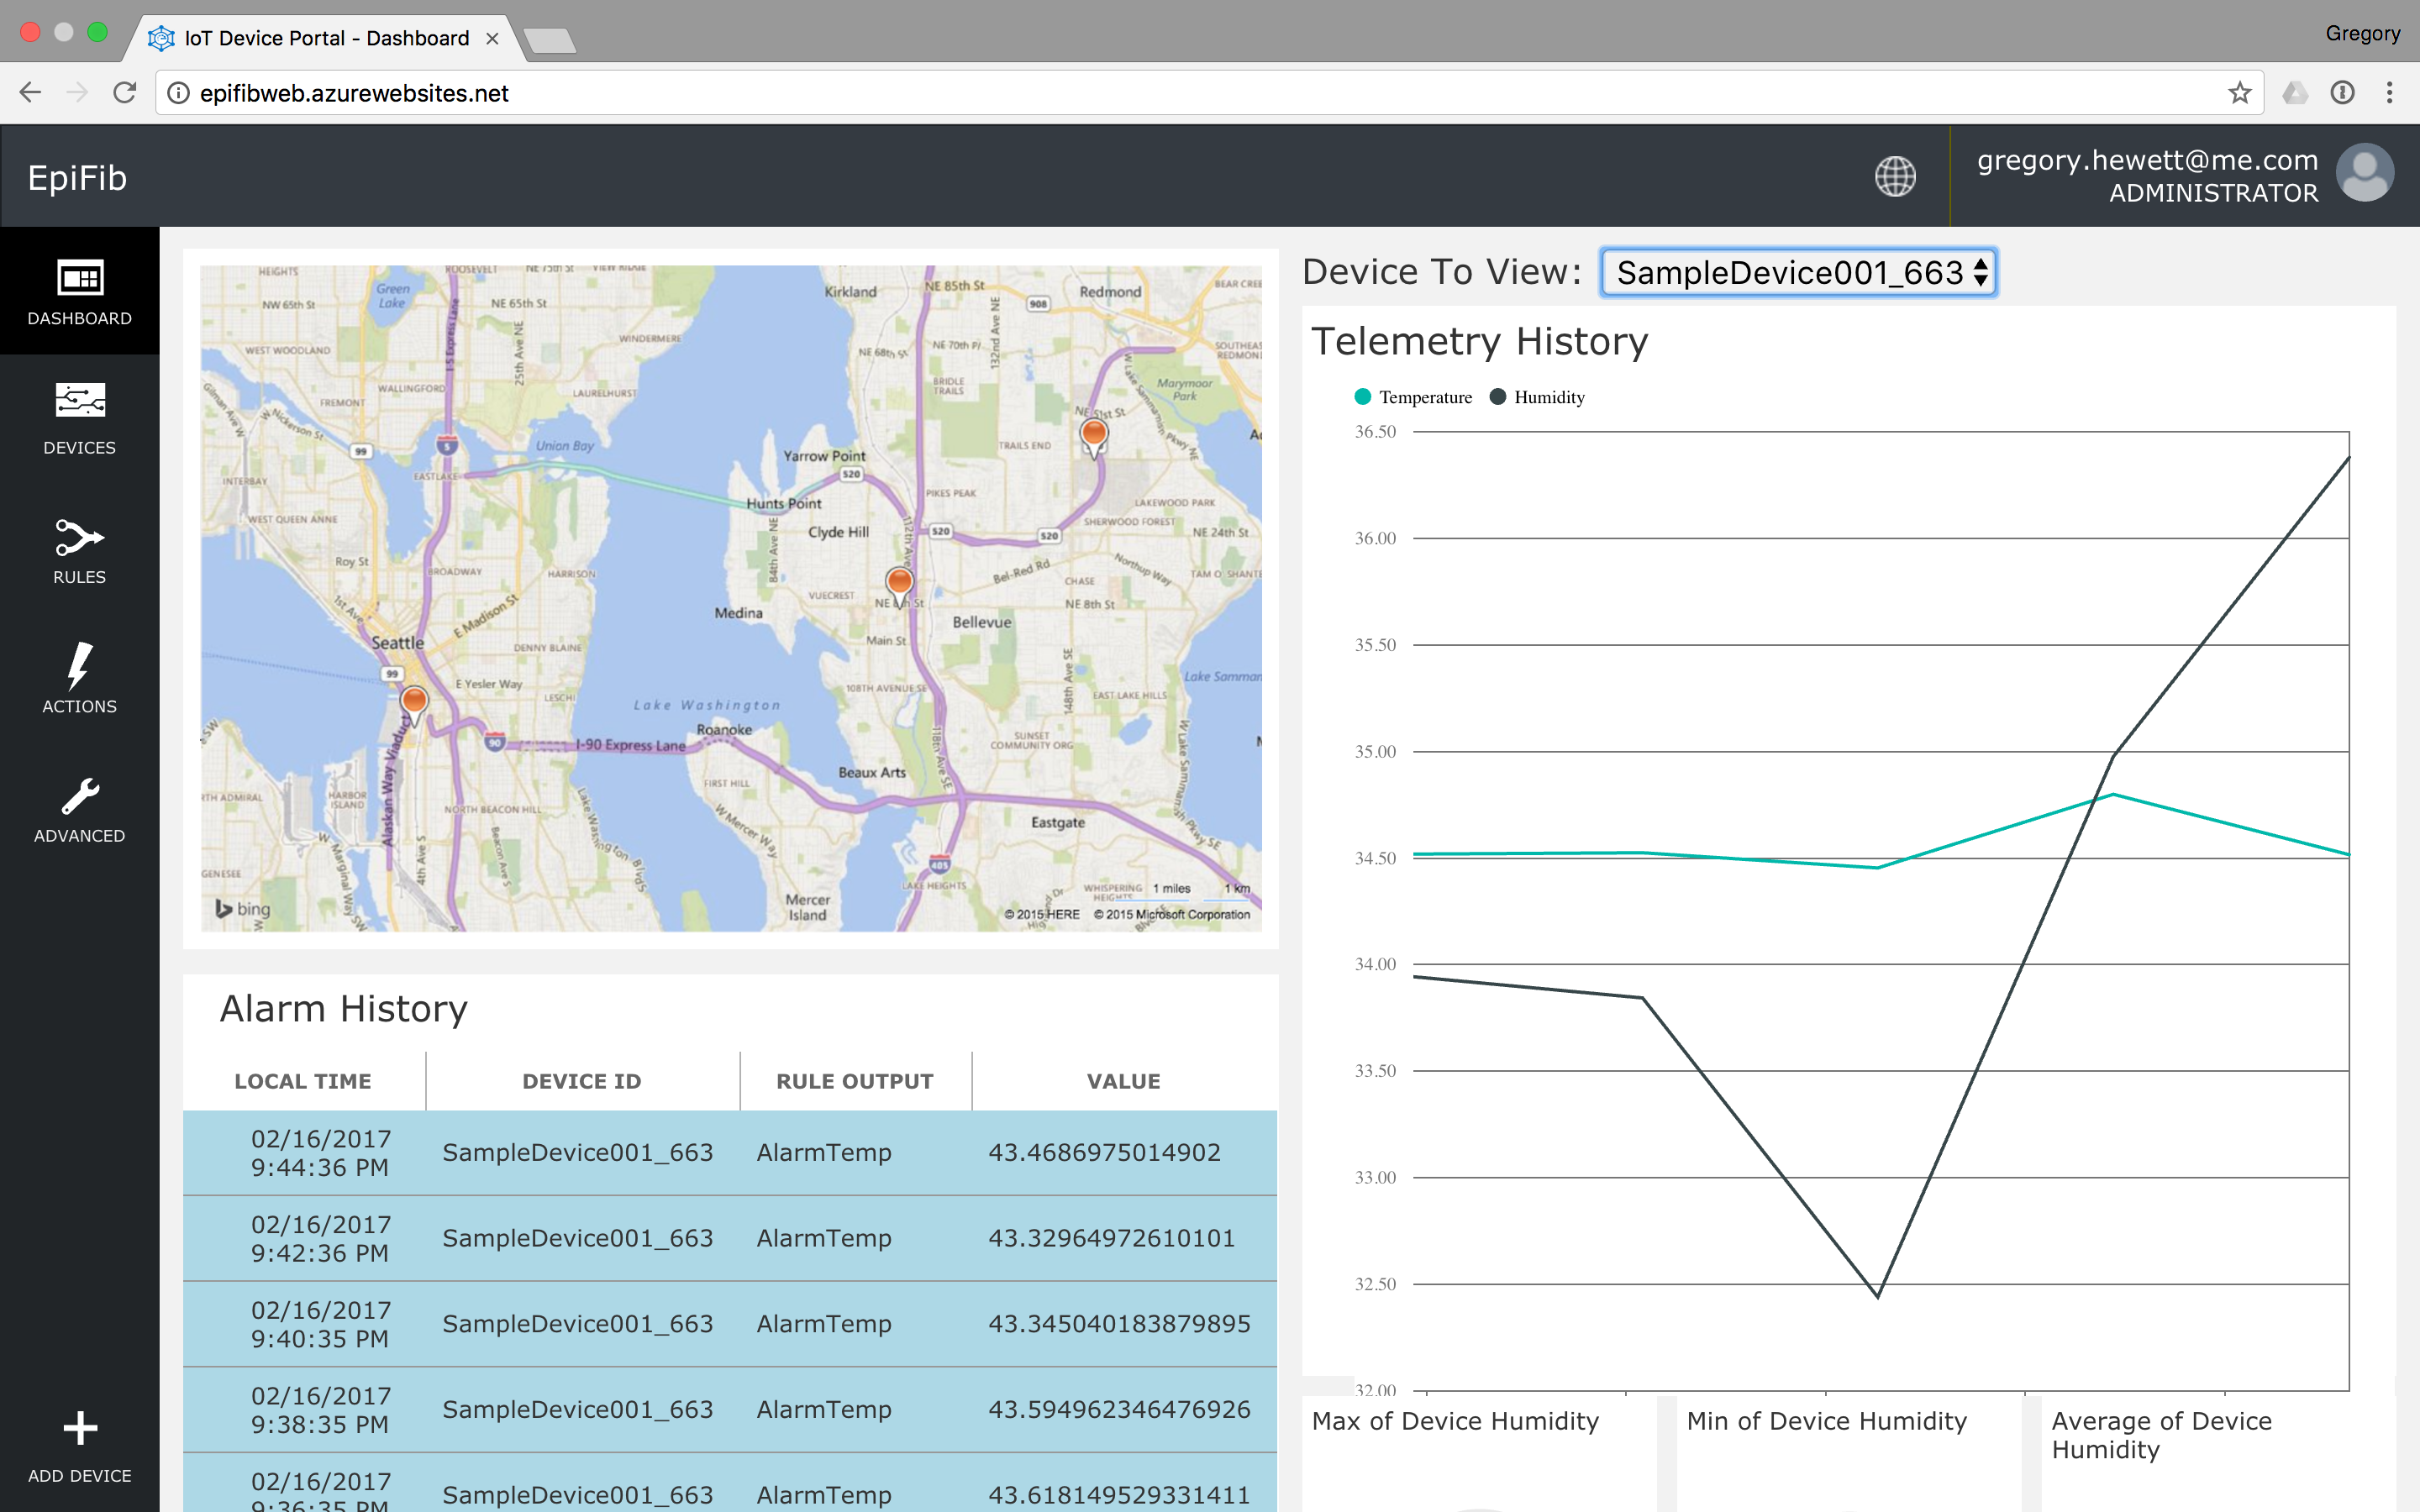
\includegraphics[width=\linewidth]{desktop-dashboard}
\caption{Container administrator dashboard for viewing container telemetry and alarm data.}
\label{fig:desktop-dashboard}
\end{figure}

\subsection{REST API and Mobile App} \label{sec:soft-design-mobile-app}

Besides device administration, the web app also contains the REST API used by the mobile app. The REST API exposes endpoints that allow a user from the mobile app to create an account, report their current location, and notify the service they need a defibrillator or autoinjector.

The mobile app provides the client-side interface for all non-administrative users. Once the user opts-in to sharing their location, the mobile app will periodically send the user's location to the service and store it using Algorithm \ref{mer-store}. Then, when a user is looking for other users with autoinjectors nearby, the user sends a request via the app, and the service notifies users nearby who can opt-in to respond.

The screenshots in Figures \ref{fig:mproto1-1-2} and \ref{fig:mproto1-3-4} show a few of the essential screens from the app. Figure \ref{fig:mproto1-1-2}(a) is the home screen. Here, a user can respond to an emergency or find an autoinjector or defibrillator.  After requesting one of these devices, in Figure \ref{fig:mproto1-3-4}(b) the user is prompted to always call 911 first before proceeding to finding users and/or containers near their location.

\begin{figure}[h]
\centering
\begin{subfigure}{.5\textwidth}
  \centering
\frame{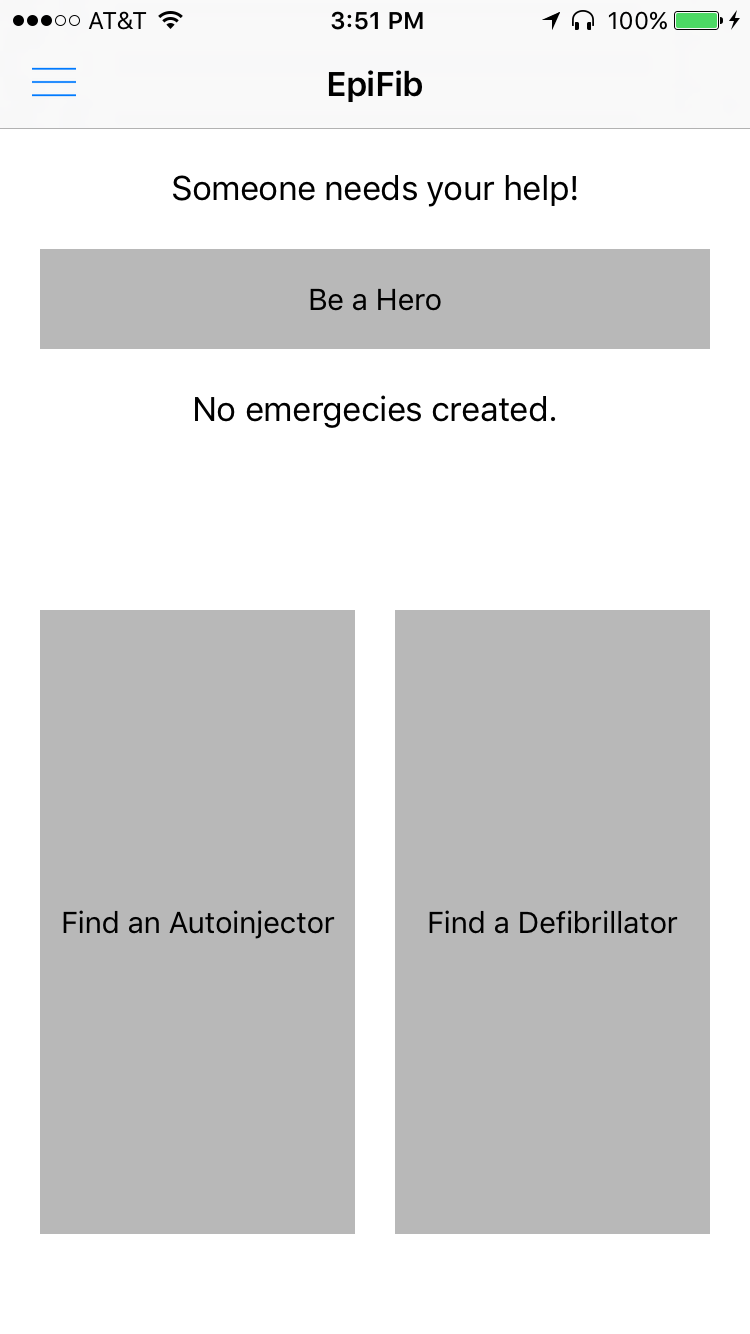
\includegraphics[height=10cm]{mobile-p1-home}}
\label{fig:mproto-1}
\end{subfigure}%
\begin{subfigure}{.5\textwidth}
  \centering
\frame{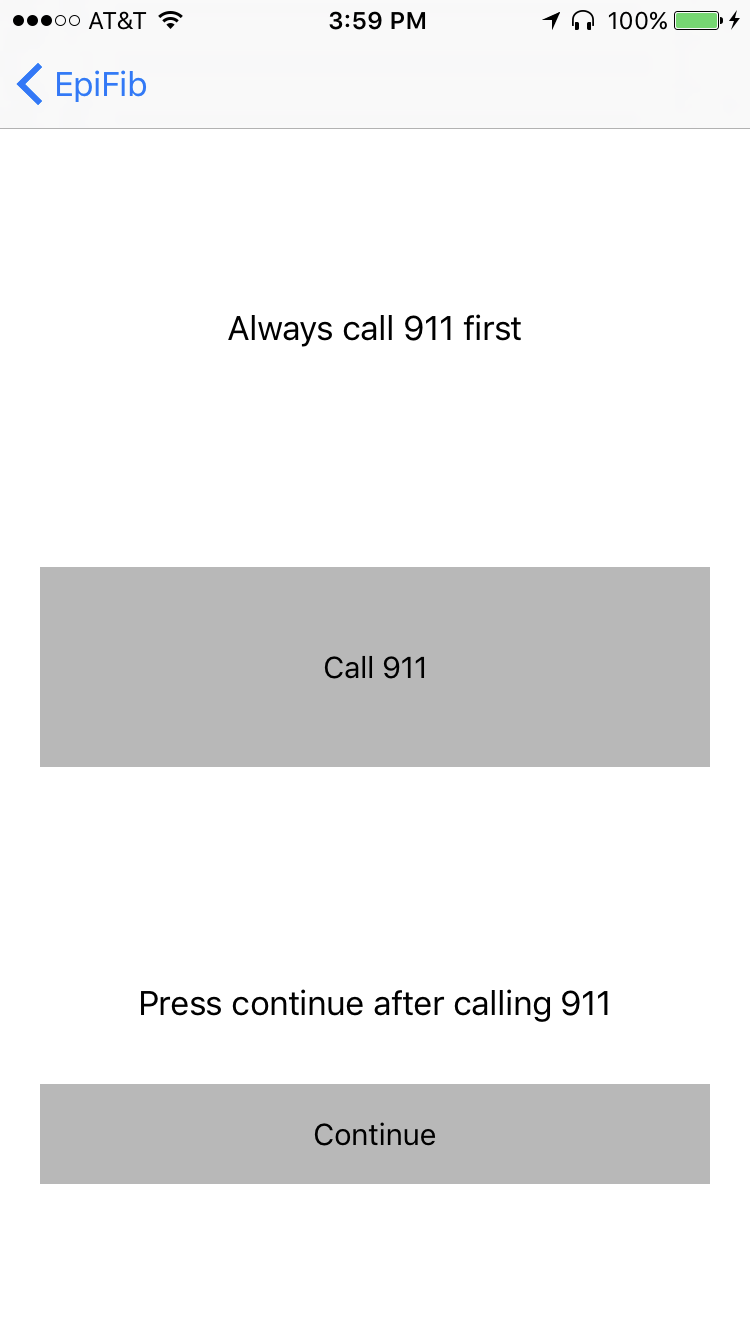
\includegraphics[height=10cm]{mobile-p1-911}}
\label{fig:mproto1-2}
\end{subfigure}
\caption{(a) Home screen and (b) after starting an emergency request, the user is prompted to first call 911.}
\label{fig:mproto1-1-2}
\end{figure}

Figure \ref{fig:mproto1-3-4}(a) shows a user looking for autoinjectors and container nearby, and Figure \ref{fig:mproto1-3-4}(b) shows the user responding to an emergency request from a user named Jennifer. More screenshots are provided in Appendix \ref{app:screenshots}.

\begin{figure}[h]
\centering
\begin{subfigure}{.5\textwidth}
  \centering
\frame{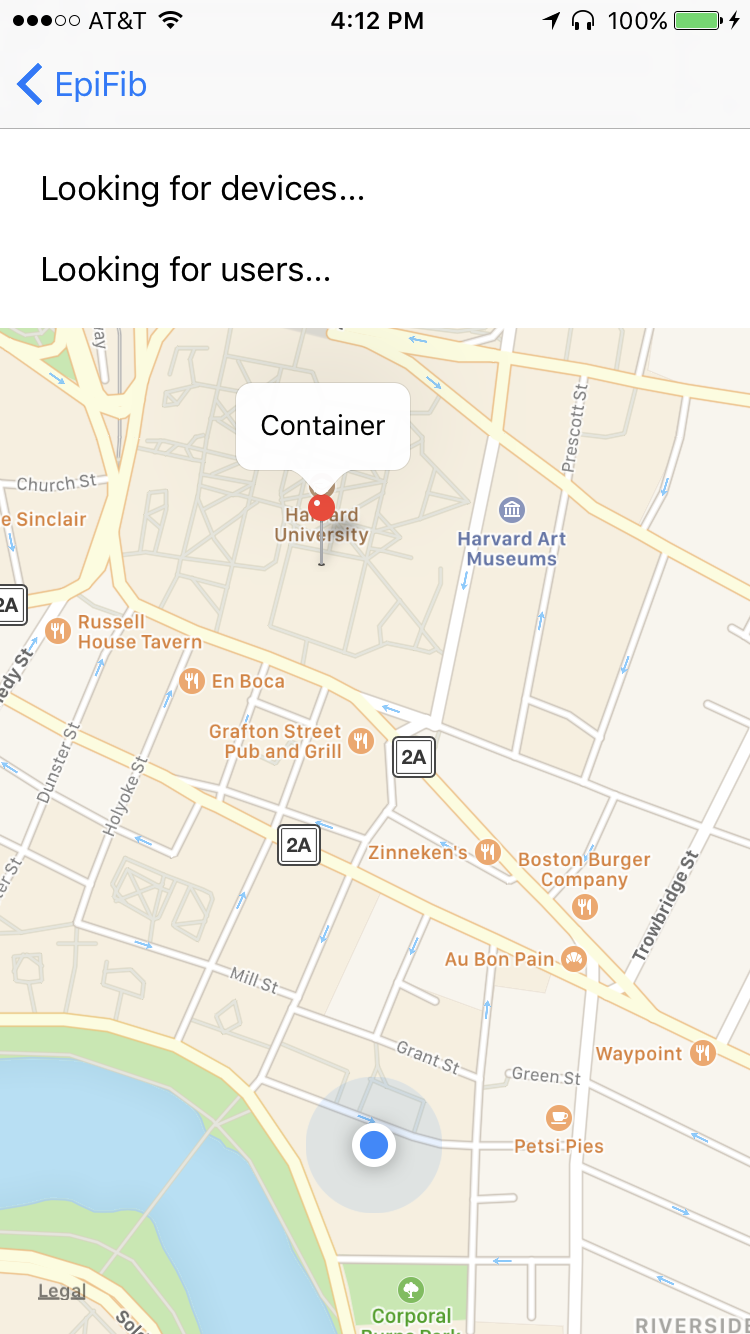
\includegraphics[height=10cm]{mobile-p1-looking}}
\label{fig:mproto1-3}
\end{subfigure}%
\begin{subfigure}{.5\textwidth}
  \centering
\frame{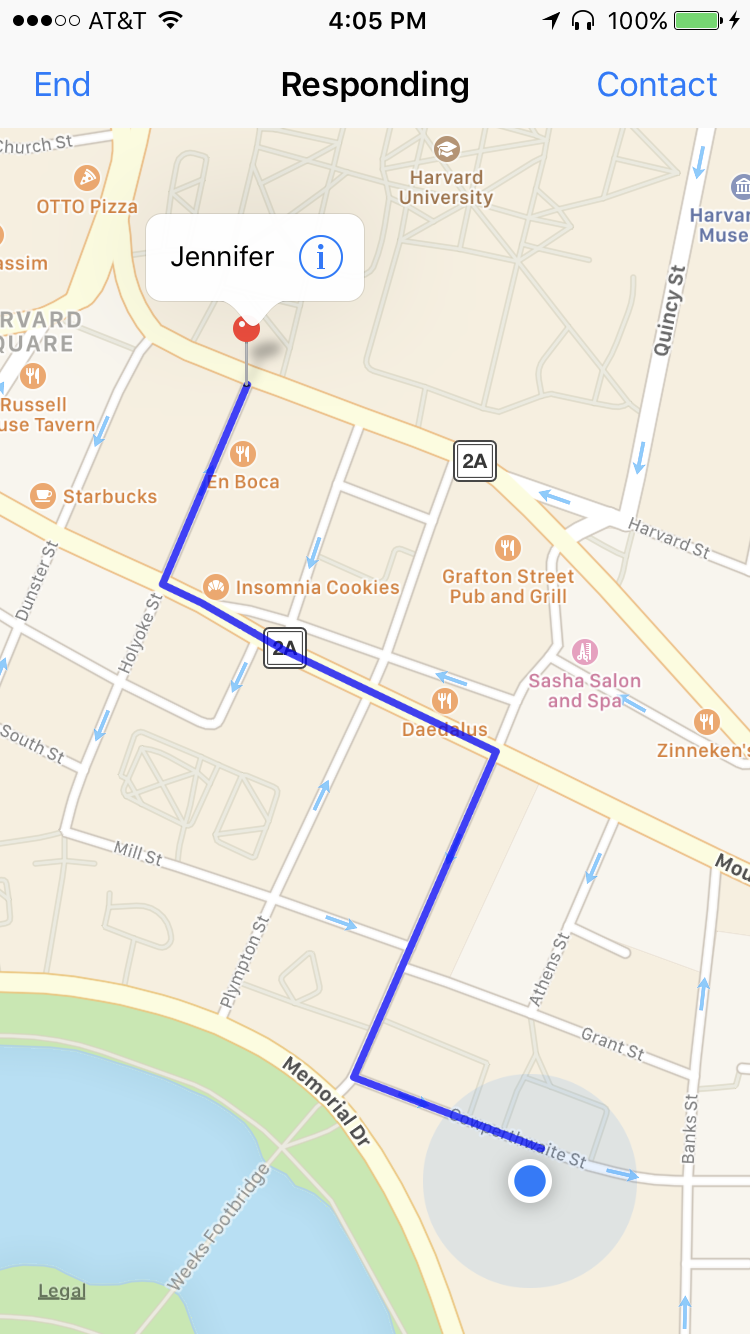
\includegraphics[height=10cm]{mobile-p1-responding}}
\label{fig:mproto1-4}
\end{subfigure}
\caption{(a) Finding nearby users and containers and (b) responding to a request from Jennifer.}
\label{fig:mproto1-3-4}
\end{figure}

\subsection{Evaluation} \label{sec:soft-eval}

The software implemented satisfies the goals presented in Section \ref{sec:soft-goals}. The container administration platform allows an administrator to add, create, update, and delete smart containers from the service. The web app and message queuing system handles all messages from smart containers efficiently, and the web app provides a simulator for simulating containers for testing.

In addition, all the mobile app goals were accomplished. Users have their own accounts and can use the app to find smart containers and autoinjectors nearby. When pinged by another user for an autoinjector, a user can navigate to someone in need.

To make this software infrastructure scalable, relevant coding and software engineering practices were used. For instance, the inversion of control paradigm was used for both the web server and mobile app design. In this model, each class or object created to perform tasks does not initialize its own dependencies. Instead, pre-initialized dependencies are taken as constructor arguments for all classes. Each class uses the objects it is passed for execution. This paradigm provides an abstraction barrier to the services used by each class, as each class is coded around its dependency interface. It also allows for easy and thorough unit testing, as mocked objects can be passed in as decencies when testing a particular class. This paradigm allows for more abstraction and a scalable infrastructure.

In addition to inversion of control, cloud-based, dynamic configuration settings are used for all database connection strings and application settings for the web app. This allows for private connection strings to be stored outside of the code base, and application settings can be changed without scheduling a new deployment. This dynamic settings are useful when an application is being used in different regions and both production and development servers are running. 

For deployment, a continuous integration protocol was used. Git was used as the version control system, and any time a new commit is pushed to the mater branch, a new deployment is triggered and all web services are updated and relaunched.











